% fig_arch (column width, 3.5 in): the detector. Source of every detail: results/research/retouch_unified_20260929/train_ru5.py
% (RUCLIP5: CLIP ViT-L/14 vision tower, frozen; LoRA r=16 on q/k/v/out projections of all 24 blocks; heads on the pooled
% feature: fz (z_f, z_b), pres (4), q (4); ev = linear on the 256 patch tokens -> 16x16 map; loss_fn incl. Addendum 46).
\documentclass[tikz,border=1.5pt]{standalone}
% Shared visual language of the TikZ figures (fig_arch, fig_system, fig_protocol, fig_exposure, fig_explain_layers).
% Colours are the palette of docs/paper_v2/figstyle.py: house blue for our model, Okabe-Ito green / vermillion for correct /
% error, light fills by stage type (network, code, language model, check, fallback, input/output), thin dark arrows.
% Text: TeX Gyre Heros (Helvetica metrics), 7 pt body; tensor shapes in DejaVu Sans Mono 5.5 pt.
\usepackage{fontspec}
\setsansfont{texgyreheros}[Extension=.otf,UprightFont=*-regular,BoldFont=*-bold,ItalicFont=*-italic,BoldItalicFont=*-bolditalic]
\setmonofont{DejaVuSansMono}[Path=/usr/share/fonts/truetype/dejavu/,Extension=.ttf,BoldFont=*-Bold,Scale=0.92]
\renewcommand{\familydefault}{\sfdefault}
\usepackage{amsmath}
\usepackage[italic]{mathastext}
\usetikzlibrary{positioning,arrows.meta,fit,backgrounds,calc,shapes.misc,decorations.pathreplacing}

% ---- palette (figstyle.py) -----------------------------------------------------------------------------------------
\definecolor{ink}{HTML}{222222}
\definecolor{muted}{HTML}{6B6B6B}
\definecolor{gridc}{HTML}{E5E5E5}
\definecolor{ours}{HTML}{0F4D92}     % house blue: our model, trainable parts
\definecolor{oursarm}{HTML}{5B9BD5}
\definecolor{okc}{HTML}{009E73}      % genuine / correct
\definecolor{errc}{HTML}{D55E00}     % forged / error
\definecolor{amber}{HTML}{C98A00}    % language model (deck palette)
\definecolor{plum}{HTML}{A8538A}     % checks
\definecolor{truth}{HTML}{56B4E9}    % ground-truth footprint
\definecolor{hilite}{HTML}{FFD700}
% light fills by stage type
\definecolor{fNet}{HTML}{E2EBF6}
\definecolor{fCode}{HTML}{DFF2EA}
\definecolor{fLLM}{HTML}{FCEFD6}
\definecolor{fChk}{HTML}{F6E6F0}
\definecolor{fFall}{HTML}{FBE4D8}
\definecolor{fIO}{HTML}{F4F4F4}

\newcommand{\bodyfont}{\fontsize{7}{8.2}\selectfont}
\newcommand{\smallfont}{\fontsize{6.2}{7.2}\selectfont}
\newcommand{\shp}[1]{{\fontsize{5.6}{6.4}\selectfont\ttfamily\color{muted}#1}}   % tensor-shape annotation
\newcommand{\hd}[1]{{\bfseries #1}}

\tikzset{
  every picture/.style={line width=0.5pt, font=\bodyfont, >={Stealth[length=3.4pt,width=2.8pt]}},
  stage/.style={rounded corners=2.2pt, draw=#1!75!black, line width=0.5pt, align=center, inner sep=2.6pt},
  net/.style={stage=ours, fill=fNet},
  code/.style={stage=okc, fill=fCode},
  llm/.style={stage=amber, fill=fLLM},
  chk/.style={stage=plum, fill=fChk},
  fall/.style={stage=errc, fill=fFall},
  io/.style={stage=muted, fill=fIO},
  plain/.style={rounded corners=2.2pt, draw=ink!55, fill=white, align=center, inner sep=2.6pt},
  flow/.style={->, draw=ink, line width=0.55pt},
  tflow/.style={->, draw=ink, line width=0.55pt, dash pattern=on 2.2pt off 1.4pt},   % training-time only
  errflow/.style={->, draw=errc, line width=0.6pt},
  okflow/.style={->, draw=okc, line width=0.6pt},
  thumb/.style={inner sep=0pt, draw=muted, line width=0.35pt},
  lbl/.style={font=\smallfont, text=ink, align=center, inner sep=1pt},
  note/.style={font=\smallfont, text=muted, align=center, inner sep=1pt},
  badge/.style={rounded corners=5pt, draw=#1, fill=white, line width=0.5pt, font=\smallfont\bfseries, text=#1, inner xsep=3pt, inner ysep=1.6pt},
}

\newcommand{\vdotsdraw}[1]{\foreach \d in {-0.07,0,0.07}{\fill[muted] ($(#1)+(0,\d)$) circle (0.45pt);}}
\begin{document}
\begin{tikzpicture}[x=1cm,y=1cm]
% ---------------------------------------------------------------- input
\node[thumb] (x) at (0.4,0.62) {
\includegraphics[width=0.75cm]{img/x.png}};
\node[lbl, anchor=south] at ([yshift=1pt]x.north) {crop $x$};
\node[anchor=north, inner sep=1.5pt] at (x.south) {\shp{224×224}};

% ---------------------------------------------------------------- backbone (24 blocks, 3 drawn)
\node[net, minimum width=2.28cm, minimum height=2.6cm] (vit) at (2.2,0.42) {};
\node[anchor=north, font=\smallfont\bfseries, text=ours] at ([yshift=-1.2pt]vit.north) {CLIP ViT-L/14};
\node[anchor=north, note] at ([yshift=-8.6pt]vit.north) {frozen, 24 blocks};
\foreach \y/\t in {0.98/1, 0.59/2, -0.10/24}{
  \node[draw=ink!40, fill=white, rounded corners=1.2pt, minimum width=2.08cm, minimum height=0.33cm] (b\t) at (2.2,\y) {};
  \node[font=\fontsize{5.4}{6}\selectfont, text=muted, anchor=center, inner sep=0pt] at (1.31,\y) {\t};
  \foreach \k/\n in {0/q,1/k,2/v,3/o}{
    \node[draw=ours, fill=fNet, line width=0.45pt, minimum size=0.23cm, inner sep=0pt, font=\fontsize{5.2}{6}\selectfont\ttfamily]
      at (1.58+\k*0.27,\y) {\n};}
  \node[draw=ink!35, fill=fIO, rounded corners=0.8pt, minimum width=0.46cm, minimum height=0.23cm, inner sep=0pt,
        font=\fontsize{5}{6}\selectfont, text=muted] at (2.88,\y) {MLP};
}
\vdotsdraw{2.2,0.30}
\node[anchor=south, align=center, font=\fontsize{5.7}{6.6}\selectfont, text=ours, inner sep=1pt] at ([yshift=1pt]vit.south)
  {{\setlength{\fboxsep}{0pt}\setlength{\fboxrule}{0.45pt}\fcolorbox{ours}{fNet}{\rule{0pt}{3.6pt}\rule{3.6pt}{0pt}}}\, LoRA rank 16, trained\\[-0.3pt]
   \textcolor{muted}{3.2\,M of 306\,M params}};
\node[anchor=north, inner sep=1.5pt] at (vit.south) {\shp{tokens 257×1024}};
\draw[flow] (x.east) -- (vit.west |- x.east);

% ---------------------------------------------------------------- heads on the pooled feature
\node[net, minimum width=4.1cm, minimum height=1.12cm] (heads) at (6.3,1.04) {};
\node[anchor=south, text=ours, font=\smallfont\bfseries, inner sep=1pt] at ([yshift=0.5pt]heads.north) {heads on the pooled feature};
\begin{scope}[every node/.style={font=\smallfont, inner sep=0.6pt}]
  \node[anchor=west] at (4.36,1.41) {$z_f$ \;forged logit};            \node[anchor=east, text=muted] at (8.24,1.41) {BCE};
  \node[anchor=west] at (4.36,1.16) {$z_b$ \;beautified logit};        \node[anchor=east, text=muted] at (8.24,1.16) {BCE};
  \node[anchor=west] at (4.36,0.91) {operation presence ×4};          \node[anchor=east, text=muted] at (8.24,0.91) {BCE};
  \node[anchor=west] at (4.36,0.66) {operation quantity ×4};          \node[anchor=east, text=muted] at (8.24,0.66) {L1};
\end{scope}
\draw[flow] (vit.east |- heads.west) -- node[above, inner sep=1pt]{\shp{CLS}} node[below, inner sep=1.2pt]{\shp{1024}} (heads.west);
\node[anchor=north, font=\fontsize{5.9}{7}\selectfont, text=ink, inner sep=1.6pt] at (heads.south)
  {decision: $P(\text{fake})=\sigma(z_f)$};

% ---------------------------------------------------------------- evidence head on the patch tokens
\node[net, minimum width=0.9cm, minimum height=0.58cm, font=\smallfont, inner sep=1pt] (evh) at (4.95,-0.5) {linear\\[-1.5pt]\shp{1024→1}};
\draw[flow] (vit.east |- evh.west) -- node[above, inner sep=1pt]{\shp{patches}} node[below, inner sep=1.2pt]{\shp{256×1024}} (evh.west);
\node[thumb] (map) at (6.12,-0.5) {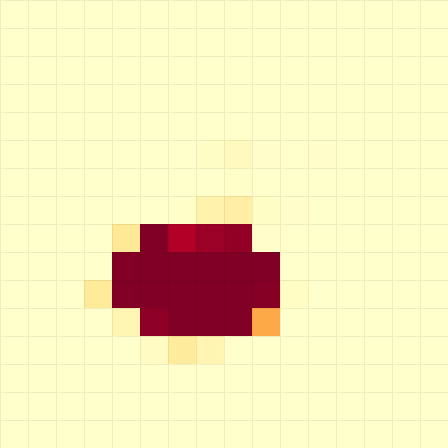
\includegraphics[width=0.72cm]{img/ev_grid.png}};
\draw[flow] (evh.east) -- (map.west);
\node[anchor=north, inner sep=1.5pt] at (map.south) {\shp{16×16}};
\node[anchor=south, lbl] at (map.north) {map $\hat m$};
\node[thumb] (fp) at (7.85,-0.5) {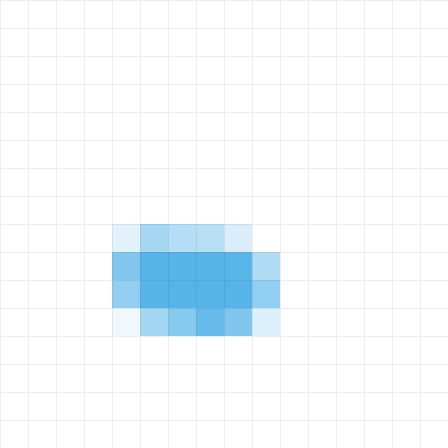
\includegraphics[width=0.72cm]{img/footprint16.png}};
\node[anchor=south, lbl] at (fp.north) {footprint $M$};
\node[anchor=north, note] at (fp.south) {exact};
\draw[<->, draw=ink, line width=0.5pt] (map.east) -- node[above, font=\fontsize{5.6}{6}\selectfont, text=muted, inner sep=1.2pt]{BCE} node[below, font=\fontsize{5.6}{6}\selectfont, text=muted, inner sep=1.2pt]{+ Dice} (fp.west);

% ---------------------------------------------------------------- training-time branch: paired smoothed view (dashed)
\node[thumb, dash pattern=on 1.6pt off 1pt, draw=ours, line width=0.5pt] (xs) at (0.4,-1.7) {
\includegraphics[width=0.75cm]{img/xs.png}};
\node[anchor=north, lbl] at ([yshift=-0.5pt]xs.south) {$x_s$,\\[-1pt]smoothed};
\draw[tflow] (xs.east) -| (0.93,-0.6) -- (vit.west |- 0,-0.6);
\node[stage=ours, fill=white, dash pattern=on 2.2pt off 1.4pt, font=\smallfont, align=left, inner sep=2.4pt, anchor=west] (cons)
  at (3.95,-1.78) {$\mathcal{L}_\text{cons}=\lambda\,\bigl(z_f(x)-z_f(x_s)\bigr)^2$,\; $\lambda$\,=\,1\\[0.2pt]
  \textcolor{muted}{$x_s$: same network; one smoothing operator}\\[-0.6pt]\textcolor{muted}{for every class; map target of $x_s$ is $M$}};
\draw[tflow] (vit.east |- 0,-0.72) -- (3.62,-0.72) |- node[pos=0.25, left, inner sep=1pt]{\shp{$z_f(x_s)$}} (cons.west);
\draw[tflow] (heads.east |- 0,1.41) -- ++(0.13,0) |- (cons.east);
\end{tikzpicture}
\end{document}
